% IF YOU ARE USING OVERLEAF, SET THE COMPILER TO XeLaTeX
% (Menu top-left > Settings > Compiler > XeLaTeX).
%
% Gemini theme — https://github.com/anishathalye/gemini  (Stanford fork)
%
% LAYOUT: ~40% (left column) is reserved for M. Vizcarra's Frontier-Curriculum half;
%         ~60% (middle + right columns) is A. Kim's ZIP-RC-Lite adaptive-compute half.
% Figures: upload the PNGs from  default_proj/ziprc_results/figures_scaled/  into a
%          ./figures/ folder in your Overleaf project (pareto_latency.png,
%          pareto_errorbars.png, calibration_auc.png).

\documentclass[final]{beamer}

% ====================
% Packages
% ====================
\usepackage[T1]{fontenc}
\usepackage{lmodern}
\usepackage[size=custom,width=120,height=72,scale=1.0]{beamerposter}
\usetheme{gemini}
\usecolortheme{stanford}
\usepackage{graphicx}
\usepackage{booktabs}
\usepackage{tikz}
\usepackage{pgfplots}
\pgfplotsset{compat=1.17}

% ====================
% Lengths
% ====================
\newlength{\sepwidth}
\newlength{\colwidth}
\setlength{\sepwidth}{0.025\paperwidth}
\setlength{\colwidth}{0.3\paperwidth}
\newcommand{\separatorcolumn}{\begin{column}{\sepwidth}\end{column}}

% ====================
% Title / authors
% ====================
\title{Frontier Curriculum and Adaptive Test-Time Compute for Efficient RLOO}

\author{Marco Vizcarra \and Andy Kim}
\institute[Stanford]{Stanford University \,---\, CS224R Final Project}

\footercontent{
  CS224R Final Project, Stanford University \hfill
  Countdown / Qwen2.5-0.5B \hfill
  \href{https://github.com/ask404/cs224r}{github.com/ask404/cs224r}}

\begin{document}

% Stanford block-S logo, top right
\addtobeamertemplate{headline}{}
{
    \begin{tikzpicture}[remember picture,overlay]
      \node [anchor=north east, inner sep=3cm] at ([xshift=0.0cm,yshift=2.5cm]current page.north east)
      {\includegraphics[height=7.0cm]{stanford_logos/Block_S_2_color.png}};
    \end{tikzpicture}
}

\begin{frame}[t]
\begin{columns}[t]
\separatorcolumn

% =====================================================================
% COLUMN 1  —  SHARED INTRO  +  MARCO'S FRONTIER-CURRICULUM HALF (~40%)
% =====================================================================
\begin{column}{\colwidth}

  \begin{block}{Introduction}
    RLOO~\cite{ahmadian2024rloo} improves reasoning on the Countdown arithmetic task, but
    vanilla RL on a 0.5B model is documented to struggle~\cite{pan2025tinyzero}. We study two
    \emph{complementary} levers for making it more efficient:
    \begin{itemize}
      \item \textbf{Part A — \emph{where} to train:} a \textbf{frontier curriculum} that
        biases RLOO toward prompts on the model's learning edge \emph{(M. Vizcarra)}.
      \item \textbf{Part B — \emph{how} to spend test-time compute:} \textbf{zero-overhead
        introspection} (ZIP-RC-Lite) that predicts reward and cost to allocate inference
        compute adaptively \emph{(A. Kim)}.
    \end{itemize}
    Both share the same SFT$\rightarrow$RLOO Qwen2.5-0.5B checkpoint and verifier.
  \end{block}

  % ===================================================================
  % MARCO: this block and the next are your ~40%. Replace / expand the
  % seed content below with your final frontier-curriculum write-up.
  % ===================================================================
  \begin{block}{Part A — Frontier Prompts \emph{(M. Vizcarra)}}
    RLOO learns best when the same prompt yields \emph{both} correct and incorrect
    completions: these ``frontier'' prompts give a clearer leave-one-out advantage than
    prompts that are always solved or always failed~\cite{chen2025sec,parashar2025e2h}.
    \begin{itemize}
      \item \textbf{Too hard:} all completions fail — little reward contrast.
      \item \textbf{Too easy:} all completions succeed — little reward contrast.
      \item \textbf{Frontier:} mixed success/failure $\Rightarrow$ useful signal
        ($0 < \texttt{success\_count} < \texttt{group\_size}$).
    \end{itemize}
    % MARCO: add method (retrieval / replay ratio) + entropy-edge baselines \cite{wu2026hive}.
  \end{block}

  \begin{block}{Frontier: Method \& Results \emph{(M. Vizcarra)}}
    % MARCO: replace this seed table with your final numbers + a plot.
    \begin{table}
      \centering
      \begin{tabular}{l r r r}
        \toprule
        \textbf{Method} & \textbf{Avg.} & \textbf{pass@1} & \textbf{pass@128} \\
        \midrule
        Vanilla RLOO         & 0.456 & 0.410 & 0.820 \\
        Frontier $r{=}0.10$  & 0.520 & 0.486 & 0.820 \\
        Goldilocks Frontier  & 0.524 & \textbf{0.493} & 0.820 \\
        Frontier continuation& \textbf{0.526} & 0.491 & \textbf{0.840} \\
        \bottomrule
      \end{tabular}
      \caption{Frontier-curriculum results (128-sample eval). \emph{Placeholder — M.V.}}
    \end{table}
    % MARCO: ablations (failure retrieval, ratios, taxonomy weighting, teacher-SFT) here.
  \end{block}

\end{column}

\separatorcolumn

% =====================================================================
% COLUMN 2  —  ANDY: ZIP-RC-LITE METHOD + CALIBRATION
% =====================================================================
\begin{column}{\colwidth}

  \begin{block}{Part B — Adaptive Test-Time Compute: ZIP-RC-Lite \emph{(A. Kim)}}
    Test-time scaling (Best-of-$N$, majority voting) spends a \emph{fixed} budget regardless
    of marginal benefit~\cite{snell2024scaling,wang2023selfconsistency}. \textbf{ZIP-RC}
    instead equips a model with \emph{zero-overhead} predictions of reward and
    cost~\cite{manvi2025zip,manvi2024adaptive}: it reuses a contiguous slice of
    \textbf{unused vocabulary logits} (Qwen2.5-0.5B has 271 free; we use ${\sim}20$) to
    output, in the \emph{same} forward pass as next-token prediction, a joint distribution
    \[
      p_\theta(\text{reward bin},\ \text{remaining length}\mid \text{prefix}).
    \]
    \textbf{ZIP-RC-Lite:} the transformer backbone is \emph{frozen}; only the reserved-logit
    head trains (cross-entropy on the joint, no KL). A live decoder then reads these
    predictions to allocate compute via meta-actions:
    \begin{itemize}
      \item \textbf{prune} trajectories predicted to fail (saves \emph{compute});
      \item \textbf{early-stop} once a trajectory is confidently correct (saves \emph{latency});
      \item \textbf{allocate} samples by predicted difficulty.
    \end{itemize}
  \end{block}

  \begin{block}{Introspection is well-calibrated}
    The head's predicted value ranks held-out rollouts by eventual correctness, and the
    \emph{live} per-step readout matches the offline scorer (works \emph{during} generation).

    \begin{figure}
      \centering
      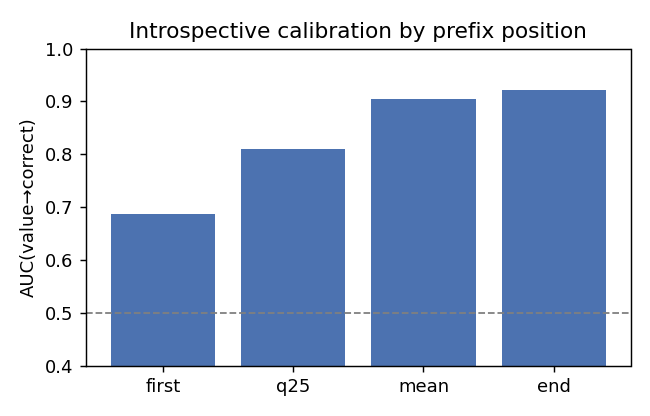
\includegraphics[width=0.78\linewidth]{figures/calibration_auc.png}
      \caption{AUC(value$\rightarrow$correct) by prefix position (held-out). Signal exists
      from the first response token.}
    \end{figure}

    \heading{Validation against the paper (K{=}64 ground-truth)}
    Our ZIP-RC-Lite calibration \textbf{matches (and beats on TV)} the values reported by
    Manvi et al.~\cite{manvi2025zip}:
    \begin{table}
      \centering
      \begin{tabular}{l c c}
        \toprule
        \textbf{Metric} & \textbf{Ours} & \textbf{Paper (ZIP-RC-Lite)} \\
        \midrule
        Mean Total Variation $\downarrow$ & \textbf{0.52} & ${\sim}0.63$ \\
        End-of-gen reward F1 $\uparrow$   & 0.81 & ${\sim}0.82$ \\
        End-of-gen reward acc $\uparrow$  & 0.67 & ${\sim}0.71$ \\
        \bottomrule
      \end{tabular}
    \end{table}
    The \emph{reward} half of the joint is well-calibrated; the \emph{length} half is weak
    (E[remaining] MAE ${\approx}257$ tokens) — an honest limitation.
  \end{block}

\end{column}

\separatorcolumn

% =====================================================================
% COLUMN 3  —  ANDY: RESULTS + SHARED CONCLUSIONS + REFERENCES
% =====================================================================
\begin{column}{\colwidth}

  \begin{alertblock}{Adaptive compute: save compute \emph{or} latency}
    The same introspection drives \emph{different} wins depending on the objective —
    the compute-vs-latency ($\alpha$) axis of~\cite{manvi2025zip}, reproduced on Countdown
    ($K{=}8$, 3 seeds, held-out):
    \begin{table}
      \centering
      \begin{tabular}{l c c c}
        \toprule
        \textbf{Policy} & \textbf{acc} & \textbf{compute} & \textbf{latency} \\
        \midrule
        none (full BoN)     & $0.708{\pm}.012$ & $3944$ & $692$ \\
        \textbf{prune}      & $0.683{\pm}.012$ & $\mathbf{1468}\ (\mathbf{-63\%})$ & $508$ \\
        \textbf{earlystop}  & $\mathbf{0.725}{\pm}.020$ & $2306$ & $\mathbf{356}\ (\mathbf{-48\%})$ \\
        \bottomrule
      \end{tabular}
    \end{table}
    \textbf{prune} cuts $\sim$63\% of compute; \textbf{early-stop} cuts $\sim$48\% of latency
    at $\geq$ baseline accuracy. The winning policy \emph{flips} with the objective.
    \begin{figure}
      \centering
      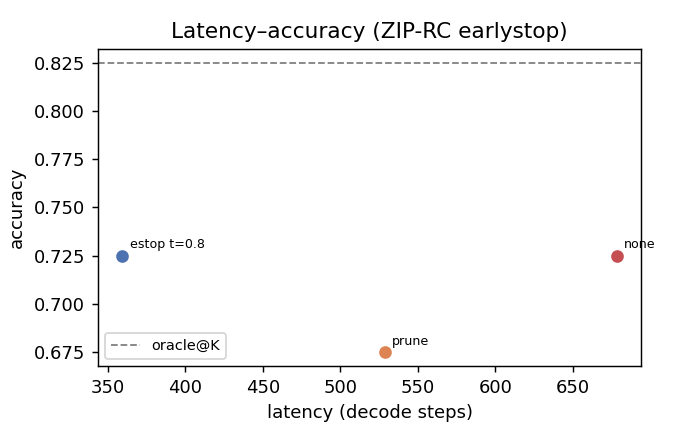
\includegraphics[width=0.72\linewidth]{figures/pareto_latency.png}
      \caption{Latency--accuracy frontier: early-stop pushes left (less latency) at or above
      the no-adaptation accuracy.}
    \end{figure}
  \end{alertblock}

  \begin{block}{Further findings}
    \begin{itemize}
      \item \textbf{Honest scoping:} value-\emph{selection} does not beat majority
        voting~\cite{wang2023selfconsistency} (value@8 $0.74$ vs majority@8 $0.78$). The
        contribution is adaptive \emph{allocation}, not better picking.
      \item \textbf{Structured 3-outcome verifier — negative, but informative:} failure-mode
        diversity is \emph{policy-capability-dependent}. Strong RLOO fails \emph{coherently}
        (3\% incoherent); weak SFT fails \emph{incoherently} (10\% coherent). No single 0.5B
        checkpoint balances all three classes, so the structured head matches binary
        (AUC $0.867$ vs $0.865$).
      \item \textbf{Cross-policy transfer:} the introspection head is largely
        \emph{policy-agnostic} — an RLOO-trained head scores SFT rollouts at AUC $0.865$
        ($\approx$ the matched SFT head's $0.867$).
    \end{itemize}
  \end{block}

  \begin{block}{Conclusions}
    \begin{itemize}
      \item \textbf{(B, A. Kim):} zero-overhead introspection on a 0.5B \emph{verifiable} task
        yields a tunable compute/latency Pareto ($-63\%$ compute or $-48\%$ latency), with
        calibration matching the original paper; the structured verifier is
        capability-dependent.
      % MARCO: add one-line conclusion for the frontier-curriculum half (A).
      \item \textbf{(A, M. Vizcarra):} frontier-prompt selection gives RLOO a clearer learning
        signal than uniform sampling. \emph{[finalize]}
    \end{itemize}
  \end{block}

  \begin{block}{References}
    \nocite{*}
    \footnotesize{\bibliographystyle{plain}\bibliography{poster}}
  \end{block}

\end{column}

\separatorcolumn
\end{columns}
\end{frame}

\end{document}
